\documentclass[english,man]{apa6}

\usepackage{amssymb,amsmath}
\usepackage{ifxetex,ifluatex}
\usepackage{fixltx2e} % provides \textsubscript
\ifnum 0\ifxetex 1\fi\ifluatex 1\fi=0 % if pdftex
  \usepackage[T1]{fontenc}
  \usepackage[utf8]{inputenc}
\else % if luatex or xelatex
  \ifxetex
    \usepackage{mathspec}
    \usepackage{xltxtra,xunicode}
  \else
    \usepackage{fontspec}
  \fi
  \defaultfontfeatures{Mapping=tex-text,Scale=MatchLowercase}
  \newcommand{\euro}{€}
\fi
% use upquote if available, for straight quotes in verbatim environments
\IfFileExists{upquote.sty}{\usepackage{upquote}}{}
% use microtype if available
\IfFileExists{microtype.sty}{\usepackage{microtype}}{}

% Table formatting
\usepackage{longtable, booktabs}
\usepackage{lscape}
% \usepackage[counterclockwise]{rotating}   % Landscape page setup for large tables
\usepackage{multirow}		% Table styling
\usepackage{tabularx}		% Control Column width
\usepackage[flushleft]{threeparttable}	% Allows for three part tables with a specified notes section
\usepackage{threeparttablex}            % Lets threeparttable work with longtable

% Create new environments so endfloat can handle them
% \newenvironment{ltable}
%   {\begin{landscape}\begin{center}\begin{threeparttable}}
%   {\end{threeparttable}\end{center}\end{landscape}}

\newenvironment{lltable}
  {\begin{landscape}\begin{center}\begin{ThreePartTable}}
  {\end{ThreePartTable}\end{center}\end{landscape}}

  \usepackage{ifthen} % Only add declarations when endfloat package is loaded
  \ifthenelse{\equal{\string man}{\string man}}{%
   \DeclareDelayedFloatFlavor{ThreePartTable}{table} % Make endfloat play with longtable
   % \DeclareDelayedFloatFlavor{ltable}{table} % Make endfloat play with lscape
   \DeclareDelayedFloatFlavor{lltable}{table} % Make endfloat play with lscape & longtable
  }{}%



% The following enables adjusting longtable caption width to table width
% Solution found at http://golatex.de/longtable-mit-caption-so-breit-wie-die-tabelle-t15767.html
\makeatletter
\newcommand\LastLTentrywidth{1em}
\newlength\longtablewidth
\setlength{\longtablewidth}{1in}
\newcommand\getlongtablewidth{%
 \begingroup
  \ifcsname LT@\roman{LT@tables}\endcsname
  \global\longtablewidth=0pt
  \renewcommand\LT@entry[2]{\global\advance\longtablewidth by ##2\relax\gdef\LastLTentrywidth{##2}}%
  \@nameuse{LT@\roman{LT@tables}}%
  \fi
\endgroup}


\ifxetex
  \usepackage[setpagesize=false, % page size defined by xetex
              unicode=false, % unicode breaks when used with xetex
              xetex]{hyperref}
\else
  \usepackage[unicode=true]{hyperref}
\fi
\hypersetup{breaklinks=true,
            pdfauthor={},
            pdftitle={Big data about small people: The Play \& Learning Across a Year (PLAY) Project},
            colorlinks=true,
            citecolor=blue,
            urlcolor=blue,
            linkcolor=black,
            pdfborder={0 0 0}}
\urlstyle{same}  % don't use monospace font for urls

\setlength{\parindent}{0pt}
%\setlength{\parskip}{0pt plus 0pt minus 0pt}

\setlength{\emergencystretch}{3em}  % prevent overfull lines

\ifxetex
  \usepackage{polyglossia}
  \setmainlanguage{}
\else
  \usepackage[english]{babel}
\fi

% Manuscript styling
\captionsetup{font=singlespacing,justification=justified}
\usepackage{csquotes}
\usepackage{upgreek}

 % Line numbering
  \usepackage{lineno}
  \linenumbers


\usepackage{tikz} % Variable definition to generate author note

% fix for \tightlist problem in pandoc 1.14
\providecommand{\tightlist}{%
  \setlength{\itemsep}{0pt}\setlength{\parskip}{0pt}}

% Essential manuscript parts
  \title{Big data about small people: The Play \& Learning Across a Year (PLAY)
Project}

  \shorttitle{PLAY Project}


  \author{Rick O. Gilmore\textsuperscript{1,3}, Karen E. Adolph\textsuperscript{2,3}, Catherine L. Tamis-LeMonda\textsuperscript{2}, Kasey Soska\textsuperscript{3}, \& Joy L. Kennedy\textsuperscript{2,3}}

  % \def\affdep{{"", "", "", "", ""}}%
  % \def\affcity{{"", "", "", "", ""}}%

  \affiliation{
    \vspace{0.5cm}
          \textsuperscript{1} The Pennsylvania State University\\
          \textsuperscript{2} New York University\\
          \textsuperscript{3} Databrary.org  }

  \authornote{
    Rick O. Gilmore is in the Department of Psychology, The Pennsylvania
    State University, University Park, PA 16802. Karen E. Adolph is in the
    Department of Psychology, New York University, 4 Washington Place, New
    York, NY 10003. Catherine L. Tamis-LeMonda is in the Department of
    Applied Psychology, New York University. Kasey Soska is is Scientific
    Project Director at Databrary. Joy L. Kennedy is Scientific Support
    Specialist at Databrary. We acknowledge support from the National
    Science Foundation (BCS-1238595), the Eunice Kennedy Shriver National
    Institute for Child Health and Human Development (U01-HD-076595), the
    Society for Research in Child Development, the Alfred P. Sloan
    Foundation, and the LEGO Foundation.
    
    Correspondence concerning this article should be addressed to Rick O.
    Gilmore, Department of Psychology, University Park, PA 16802. E-mail:
    \href{mailto:rogilmore@psu.edu}{\nolinkurl{rogilmore@psu.edu}}
  }


  \abstract{Piaget, Montessori, and Bruner observed that play is the work of
infants. The PLAY (Play \& Learning Across a Year) project seeks to
catalyze discovery about the form and dynamics of this essential work
across a critical period from 12 to 24 months of age when infants show
remarkable advances in language, object interaction, locomotion, and
emotion regulation. PLAY will leverage the joint expertise of 65
``launch group'' researchers and capitalize on the Databrary
video-sharing library and Datavyu video-coding tool to exploit the power
of video to reveal the richness and complexity of behavior. The PLAY
researchers will collect, transcribe, code, share, and exploit a video
corpus of infant and mother naturalistic activity in the home to test
hypotheses about behavioral, developmental, and environmental cascades.
In turn, the project will demonstrate the value and feasibility of a
cross-domain synergistic approach to infant research while advancing new
ways to use video as data and documentation to facilitate discovery and
ensure transparency.}
  \keywords{keywords \\

    \indent Word count: X
  }





\usepackage{amsthm}
\newtheorem{theorem}{Theorem}[section]
\newtheorem{lemma}{Lemma}[section]
\theoremstyle{definition}
\newtheorem{definition}{Definition}[section]
\newtheorem{corollary}{Corollary}[section]
\newtheorem{proposition}{Proposition}[section]
\theoremstyle{definition}
\newtheorem{example}{Example}[section]
\theoremstyle{definition}
\newtheorem{exercise}{Exercise}[section]
\theoremstyle{remark}
\newtheorem*{remark}{Remark}
\newtheorem*{solution}{Solution}
\begin{document}

\maketitle

\setcounter{secnumdepth}{0}



Behavior lies at the core of developmental science (Gibson, 1994). Video
is a uniquely powerful tool for capturing the richness and complexity of
behavior (K. E. Adolph, Gilmore, \& Kennedy, 2017; Rick O Gilmore \&
Adolph, 2017), documenting its microstructure in real time and global
patterns of change over development (Gesell, 1946, 1991). Video
chronicles who did what, and how, when, and where they did it (K. E.
Adolph et al., 2017; Gilmore \& Adolph, n.d.; Rick O Gilmore, Adolph,
Millman, \& Gordon, 2016). Most infancy researchers collect video as
primary data or as a backup to online coding procedures, but until
recently, few have openly shared video because of ethical and technical
challenges. As those challenges recede and the culture of developmental
science begins to embrace more open, transparent, and reproducible
practices (Frank et al., 2017), the time is ripe to capitalize on the
unique power of video to catalyze discovery and transform knowledge
about behavioral development in infancy.

The Play \& Learning Across a Year (PLAY) project (K. E. Adolph,
Gilmore, \& Tamis-LeMonda, 2016, 2018) builds on the NICHD/NSF-funded
Databrary video-sharing library (``Databrary,'' n.d.; Gilmore, Adolph,
\& Millman, 2016) and the Datavyu video-coding tool (K. E. Adolph, 2015;
``Welcome!~\textbar{}\textbar{}~datavyu,'' n.d.) developed and supported
by Adolph and Gilmore, and it unites the joint expertise of 65 PLAY
\enquote{launch group} researchers in the United States and Canada. PLAY
will create the first-of-its-kind, large-scale, openly shared, readily
reusable, transcribed, coded, and curated video corpus of human
behavior. In addition, PLAY seeks to advance new video-based means of
research documentation that hold promise to increase transparency and
bolster reproducibility (K. E. Adolph et al., 2017; Rick O Gilmore \&
Adolph, 2017) across the behavioral sciences. In this paper, we describe
the process of planning PLAY, our preliminary results from a small pilot
study, and plans for a larger scale implementation we expect to launch
in late 2018.

\section{Project Planning}\label{project-planning}

\subsection{Why's and wherefore's}\label{whys-and-wherefores}

We named the project \enquote{PLAY} and use the terms
\enquote{unstructured play} and \enquote{everyday play} to broadly refer
to infants' natural activities while awake. To paraphrase Piaget
(Piaget, 1967), Montessori (Montessori, 1984), and Bruner (Jerome S
Bruner, 1975; Jerome Seymour Bruner, 1976), play is the work of infants.
It is an approach to action, not a particular form of activity. Some of
infants' play involves toys and some play is joyful and goal directed,
but all of their spontaneous vocalizations, interactions with objects
and people, and locomotor bouts involve exploration and opportunities
for learning and growth, regardless of affect or intent.

\subsection{Recruiting the launch
group}\label{recruiting-the-launch-group}

Planning for the project began in late 2015. Adolph, Tamis-LeMonda and
Gilmore (PLAY PIs) invited researchers to join the launch group based on
their interest in open science and infant-mother natural activity in the
home, willingness to collaborate on data collection and coding, lab
location, and domains of expertise (language, gesture, play, object
exploration, tool use, locomotion, posture, physical activity, emotion,
temperament, parent responsiveness, gender, home environment, media use,
spatial demography, and sampling). Nearly every invitee agreed. As of
Spring 2018, the current launch group consists of 65 researchers from 49
institutions and 24 states. 34\% are new investigators, 68\% women, 18
non-white, from varied institutions (public and private universities and
colleges, hospitals, agencies) with varied resources (38 public
universities, 18\% R15-eligible institutions) across the United States
and Canada.

To distribute the burden of video coding across researchers, we
recruited more than 10 experts to shape the development of coding passes
in four fundamental domains--communication, object interaction,
locomotion, and emotion. These domains represent key areas of infant
development and provide foundational information for future discovery
when time-locked to video.

\subsection{Launch group deliberations and
decisions}\label{launch-group-deliberations-and-decisions}

Through a yearlong series of telephone conversations with each launch
group member and 12 group webinars (K. E. Adolph, Tamis-LeMonda, \&
Gilmore, n.d.), we jointly developed a common sampling method and
protocol (including materials, technical specifications, questionnaires,
and non-video measures), designed common video codes, and established an
infrastructure to divide responsibilities between PLAY staff and launch
group. We achieved consensus, with input from NICHD program staff, about
all aspects of PLAY at a daylong workshop at NIH in December 2016,
materials from which are shared on Databrary (K. E. Adolph et al.,
2016).

The launch group jointly decided that the centerpiece of PLAY would be
900 one-hour videos of infant-mother dyads during natural play in the
home. Home videos are widely believed to be representative of natural
activity, and provide a stark contrast to the 2- to 20-minute
\enquote{snapshots} typical of standard structured lab tasks. Based on
their extensive experience with naturalistic home observations (Barbaro,
Johnson, Forster, \& Deák, 2015; Fausey, Jayaraman, \& Smith, 2016;
Iverson \& Wozniak, 2007; Karasik, Adolph, Tamis-LeMonda, \& Zuckerman,
2012; Karasik, Tamis-LeMonda, \& Adolph, 2011; Karasik, Tamis-Lemonda,
\& Adolph, 2014; Karasik, Tamis-LeMonda, Adolph, \& Bornstein, 2015;
Rowe, 2012; Soderstrom \& Wittebolle, 2013), launch group members
determined that one hour is sufficiently long to capture an ecologically
valid window into infant and mother natural behaviors. Longer recording
times produce diminishing returns, risk infants becoming excessively
tired or hungry, and increase the cost and burden to families and
researchers.

The launch group determined the specific foundational codes to be
applied to the videos in each of the domains of language and
communication, locomotion and physical activity, object interaction, and
emotional expression. The foundational codes were chosen to be
informative even to non-experts and were designed to facilitate further
discovery through subsequent coding passes that build on the prior work.
The codes were intendd to be quick, easy, and reliable to code in
comparison with some other behaviors (e.g., visual attention) \emph{not}
chosen for coding. Temporally aligned transcriptions and codes should
enable researchers with expertise in any domain to analyze cascades
within and among these behaviors. Experts in language and communication
also recommended that we transcribe all mother speech and infant
vocalizations in formats exportable to CHILDES (MacWhinney, 2000a).

Given the cost of going to families' homes, the launch group determined
that we should augment recordings of natural play with a set of
additional video, questionnaire, and non-video measures, that together
would add only \textasciitilde{}45 minutes to the home visit. This would
enable researchers to test whether variations in natural play, or in
characteristics of distal and proximal environments, predict infant and
mother behaviors when materials and conditions are held constant. Thus,
the solitary and dyadic play tasks are of interest in their own right,
and might also serve as correlates in tests of experiential and
environmental influences.

To obtain objective data on stable home conditions (cracks in walls,
broken windows, ceiling stains, safety issues, etc.), physical layout
(furniture, clutter, space to move, etc.), educational and electronic
media (writing/drawing materials, TVs, computers, etc.), and gendered
characteristics of infants' room, toys, and clothes, we decided to
conduct video home tours. Launch group experts also expressed interest
in understanding whether clothing and footgear affect infants'
locomotion and physical activity, and each takes only moments to video
record. Clothing/footgear videos can reveal gendered features
(bows/frills, superhero emblems, patent leather shoes, army boots)
(Halim, Ruble, Tamis-LeMonda, \& Shrout, 2013) and influences on
spontaneous activity and locomotion (Cole, Lingeman, \& Adolph, 2012).
The launch group also deemed important a variety of questionnaire
measures of infant skills, experiences, and home environment: mothers'
report of infants' vocabulary, locomotor milestones and falls,
temperament, and use of gender labels; mother's report of family
demographics, media use, health, and home chaos; and a
researcher-completed survey on physical characteristics of the home. The
PIs developed a custom tablet-based app to collect these questionnaire
data efficiently, limit data input errors, use a stylus for flexible
data entry, and allow automatic transfer to permanent storage on
Databrary. The launch group devised methods to measure room size with a
commercial laser device and ambient noise level with a commercial
decibel meter.

\section{Pilot Study}\label{pilot-study}

Based on the launch group's initial recommendations, we carried out a
pilot study in the New York City area to test the feasibility of the
approach. We chose to recruit infants at 12-, 18-, and 24-months because
12- to 24-months represents a period of important, rapid growth when
children begin talking, using objects in symbolic play, walking, and
regulating emotions. For example, by 12 months, about half of infants
can walk and half still crawl. By 18 months, infants are proficient
walkers, and by 24 months, they can run, walk backwards, and walk up
stairs (Onis, 2006; Robinson, 2015). Around 12 months, infants produce
their first words. By 18 months, most display a vocabulary spurt, and by
24 months infants combine words into simple sentences (Bloom, 1995;
Hoff, 2013). But these ages represent only group averages; individual
infants show tremendous variability in these behaviors at each age.

\subsection{Methods}\label{methods}

\subsubsection{Participants}\label{participants}

A total of \(n=\) 20 infants were tested, \(n=\) 4 12-month-olds (3
female), \(n=\) 12 18-month-olds (5 female), and \(n=\) 4 (0 female)
24-month-olds.

All infants recruited were from the New York City area. Fifteen infants
were White, one was Asian, two reported more than one race, and two did
not report a race. Six were of Hispanic or Latino ethnicity.

\subsubsection{Procedure}\label{procedure}

During an initial screening call, a researcher determined eligibility
for participation and obtained demographic information. The researcher
scheduled a 2-hour visit (weekday or weekend) when infants were to be
between naps, meals, and baths, and would normally be home with their
mothers.

The visit included parent consent, one-hour natural play, two structured
play tasks, questionnaires, video home tour, and Databrary sharing
permission. Although mothers were asked to agree to share data in the
initial screening call, we requested their signed permission at the end
of the home visit when they were maximally informed about the procedures
that had taken place. If families decline to share, their data were
still be stored on Databrary as \enquote{Private} and thus available for
use only by the collecting researchers for their own purposes. Consent,
sharing permission, and questionnaire data were entered on a custom
Android tablet app; paper forms and video camera on tripod provided
backup.

During the visit, we recorded one hour of infant and mother activity in
the home. Infant and mother went about their daily routines without
restrictions. They could move from room to room; mother could do chores;
TV, music, or other media could be on. The researcher held an HD video
camera at the child's eye level, prioritizing view of infant over
mother, keeping the infant's face, hands, and feet in view. If mother
was visible, the researcher captured as much of her face and body as
possible without losing view of the baby. A cardioid microphone
amplified infant and mother speech and isolated background noise.

Two structured play tasks followed the one hour of natural activity.
Solitary play entailed infants playing with a set of 10 nesting cups
(placed half up, half down) while sitting on a mat with mother nearby
but not interacting (2 minutes). In dyadic play infant and mother played
together on the mat with a standard set of toys (3 minutes)-- truck,
doll, baby bottle, small blanket, 2 tea cups, plates, and spoons---with
mother instructed to \enquote{share the toys with her child.} The toys
were thought to be conducive to non-symbolic (stacking plates, cups),
symbolic (feeding doll, putting doll to sleep), and gendered play (with
truck versus doll).

Following the play episodes, the researcher walked through each room,
recording walls, floors, ceilings, windows, room contents (including
infants' toys, books, media), and the contents of infants' closets and
drawers. The mother was asked to name each room, describe infant's
access to rooms and spaces, and open closet doors and drawers for
recording. Prior work gave us confidence that mothers would not find
this procedure intrusive. The researcher narrated the video with
comments about floor coverings (\enquote{throw rug,} \enquote{linoleum})
and anything not transparent to video.

In addition, during the visit the researcher recorded the clothes (front
and back) and footgear (bottom, side, top) infants wore during the
natural play session, and recorded the date infants began wearing the
shoes and for how many days/week infants play indoors in shoes, socks,
and barefoot.

After the naturalistic and structured play tasks, the researcher
interviewed mothers on a range of infant and family measures that will
yield information about language, locomotion, temperament, gender, home
environment, and health. The researcher administered all questionnaires
orally, and video records the interview (camera on tripod) for quality
assurance, transparency, and possibly later coding.

At the end of the visit, the researcher asked mothers if the one-hour
natural play session was representative of a typical day at home. If
mothers reported that infants' behavior or health was atypical, we would
have replaced the dyad and documented the replacement.

A publicly-accessible wiki (Soska, Adolph, Tamis-LeMonda, \& Gilmore,
2016) was used to document all procedures and code definitions. The wiki
links descriptions of every aspect of the protocol with exemplar
third-person video clips (e.g., researcher scheduling home visit) to
demonstrate typical procedures. The wiki links text-based descriptions
of each code to video clips illustrating the types of behaviors that do
and do not satisfy the coding criteria.

\subsubsection{Data analysis}\label{data-analysis}

For this report, we used R (Version 3.4.4; R Core Team, 2017) and the
R-packages \emph{acs} (Version 2.1.3; Glenn, 2018), \emph{bindrcpp}
(Version 0.2.2; Müller, 2016), \emph{choroplethr} (Lamstein, 2017;
Version 3.6.1; Lamstein \& Johnson, 2017), \emph{choroplethrMaps}
(Version 1.0.1; Lamstein, 2017), \emph{chron} (Version 2.3.52; James \&
Hornik, 2018), \emph{databraryapi} (Version 0.1.2.9002; Rick O. Gilmore,
21AD), \emph{dplyr} (Version 0.7.4; Wickham \& Francois, 2016),
\emph{forcats} (Version 0.3.0; Wickham, 2018a), \emph{ggmap} (Version
2.7.900; Kahle \& Wickham, 2013), \emph{ggplot2} (Version 2.2.1;
Wickham, 2009), \emph{httr} (Version 1.3.1; Wickham, 2017a),
\emph{jsonlite} (Version 1.5; Ooms, 2014), \emph{papaja} (Version
0.1.0.9709; Aust \& Barth, 2017), \emph{purrr} (Version 0.2.4; Henry \&
Wickham, 2017), \emph{readr} (Version 1.1.1; Wickham, Hester, \&
Francois, 2017), \emph{stringr} (Version 1.3.0; Wickham, 2018b),
\emph{tibble} (Version 1.4.2; Wickham, Francois, \& Müller, 2017),
\emph{tidyr} (Version 0.8.0; Wickham, 2017b), \emph{tidyverse} (Version
1.2.1; Wickham, 2017c), and \emph{XML} (Version 3.98.1.10; Lang \& CRAN
Team, 2018) for all of our statistical analyses. Datavyu
(``Welcome!~\textbar{}\textbar{}~datavyu,'' n.d.) was used for video
coding. All code used in data analysis and for this manuscript may be
found in the GitHub repository associated with the paper (``PLAY project
protocol manuscript,'' n.d.).

To compute inter-observer reliability, we ran scripts in Datavyu to
selects a random segment of video (25\% or 5 mins) from each 20- minute
segment of natural play. Inter-observer reliability for the pilot videos
was 96.7\%-99.3\% exact frame agreement (\(\kappa\)s \textgreater{} .93,
\(ps\) \textless{} .001) for duration codes (object interactions,
locomotion, emotion) and 94.1\%- 99.5\% code agreement (\(\kappa\)s
\textgreater{} .89, \(ps\) \textless{} .001) for categorical events
(communicative acts, gesture).

\subsection{Results}\label{results}

Our pilot tests verified the feasibility of collecting all data in less
than 2 hours. So, with 1-2 hours of round-trip travel time, the entire
data collection could be completed in less than 4 hours.

Informal inspection of the videos verified that dyads were unaffected by
the presence of the researcher: After a few minutes of acclimation prior
to natural play, mothers and infants ignore the researcher. Infants
cried and breastfed; mothers yelled, talked on the phone, worked on
computers, went about daily chores, changed infants' diapers, and gave
infants snacks. Mothers appeared comfortable with all procedures,
including the video home tour. The PIs found wide variation in home
\enquote{disarray,} suggesting parents present homes as they would for
any other casual visitor.

All families were asked permission to share data with authorized
researchers on Databrary using language adapted from the Databrary
release template (Rick O. Gilmore \& Adolph, n.d.). Nineteen of the 20
families agreed to share; 3 families agreed to share data only with
authorized Databrary researchers and 16 agreed to allow authorized
researchers to show clips in public settings for informational or
educational purposes.

In carrying out detailed video coding on 4 of the participants'
sessions, we established that all four foundational coding passes are
easy to learn (by undergraduate coders on Datavyu) and time efficient
(\textless{} 3 hours for both infant and mother for each coding pass per
hour of video). Adaptations to Datavyu enable transcription in English
or Spanish to take 7-9 hours per hour of video, while infant and mother
communicative acts and gestures together take \textless{} 3 hours to
code.

\subsubsection{Demographic and self-report
measures}\label{demographic-and-self-report-measures}

Due to some technical difficulties with pilot versions of the tablet
app, we are only able to report here demographic and self-report data
from \(n=\) 18 families. Reconstructions of the missing data from video
are ongoing, and updates will appear on the project's Databrary volume
(Adolph, Tamis-LeMonda, \& Gilmore, n.d.) once those are completed.

\begin{figure}

{\centering 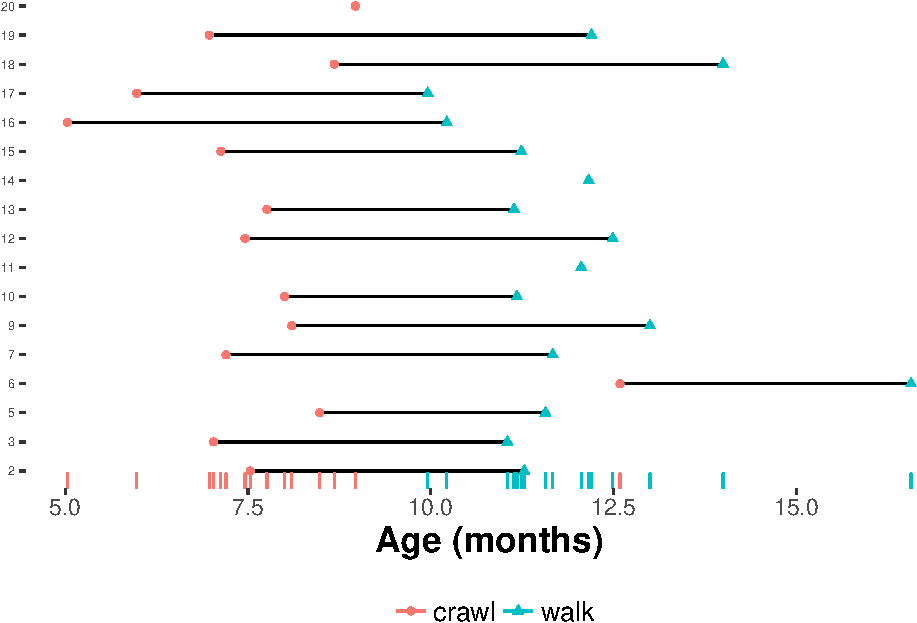
\includegraphics{ibad-ms_files/figure-latex/locomotion-plot-1} 

}

\caption{Parent-reported onset ages for hands and knees crawling and walking}\label{fig:locomotion-plot}
\end{figure}

Infants had largely uncomplicated, healthy births. Birth weights (in g)
ranged from 2,721.55 to 4,025.63 (mean = 3,495.58 g); 3 had birth
complications (e.g., C-section, preeclampsia). Figure
@ref\{fig:locomotion-plot\} shows the parent-reported ages for the onset
of hands and knees crawling and walking using procedures Adolph has used
previously (Adolph et al., 2012; Adolph, Vereijken, \& Shrout, 2003).

Mothers reported having between 17 and 23 years of education, (\(M=\)
20.50) and 15 were working at least part time. Sixteen of the eighteen
repondents reported a partner cohabitating with the family. The
partner's education level ranged from 17 and 23 years of education,
(\(M=\) 20.60) and 15 were working at least part time.

All of the infants were exposed to and spoken to in English in the home.
Many were spoken to or had exposure to languages other than English. At
home 4 infants were spoken to in Spanish; 3 infants were exposed to
Spanish in a childcare setting. Other children were exposed to Armenian,
French, Hindi, Polish, and Russian in the childcare setting. Six
children in this sample were exposed only to English.

\subsubsection{Video coding}\label{video-coding}

NEED figures here.

\subsection{Discussion}\label{discussion}

The pilot study verified that the protocol met the launch group's
criteria on scientific and practical grounds. Four of the full sessions
(cases 13, 18, 29, and 20) met all internal criterion benchmarks. These
were used to populate the wiki (Soska et al., 2016) with illustrative
exemplars of procedures and code definitions.

\section{Planned study}\label{planned-study}

The proposed full study builds upon and extends the pilot (K. E. Adolph
et al., 2016, 2018) study. We described the details in a grant proposal
to NICHD submitted in June 2017 that was reviewed in October 2017. The
proposal received a 1st percentile in peer review, and as of April 2018,
we are awaiting a formal Notice of Award.

\subsection{Methods}\label{methods-1}

\subsubsection{Participants}\label{participants-1}

\begin{figure}

{\centering 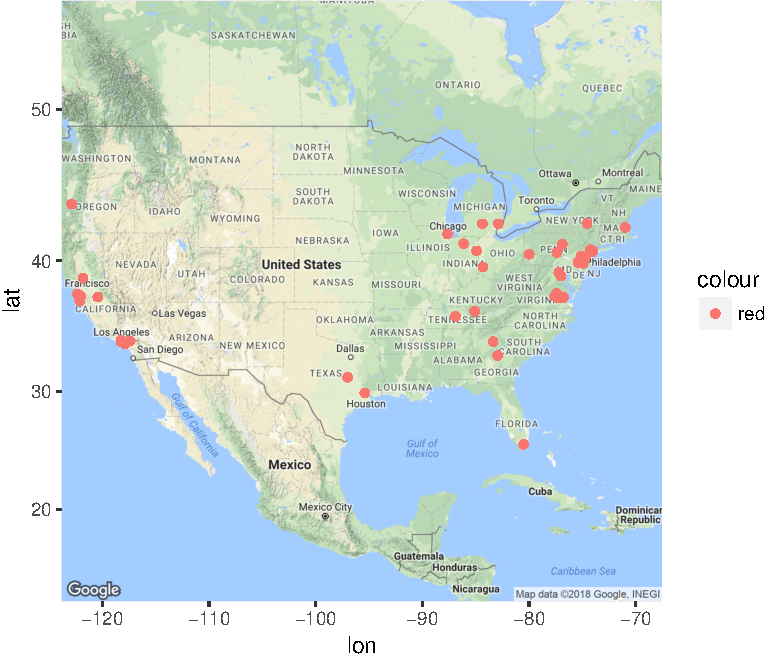
\includegraphics{figs/PLAY-collection-map-1} 

}

\caption{Map of planned data collection sites for PLAY project.}\label{fig:play-site-map}
\end{figure}

We will collect data from \(n=900\) infant-mother dyads from 30
different communities in 17 states located around the U.S. Each site
will collect data from 30 infants, 10 each at 12-, 18-, and 24-months of
age (+/- 1 week), with equal numbers of females and males. Figure
@ref\{fig:play-site-map\} shows a map of the proposed data collection
sites.

While not designed to be nationally representative, the data collection
sites are diverse in aggregate based on Census data. To gather Census
data reproducibly, we used the \texttt{choroplethr} package (Lamstein,
2017; Lamstein \& Johnson, 2017) to download data from the Census
Bureau's public API. This workflow allows us to easily gather and
analyze other Census Bureau data about the communities targeted for
sampling.

\begin{figure}

{\centering 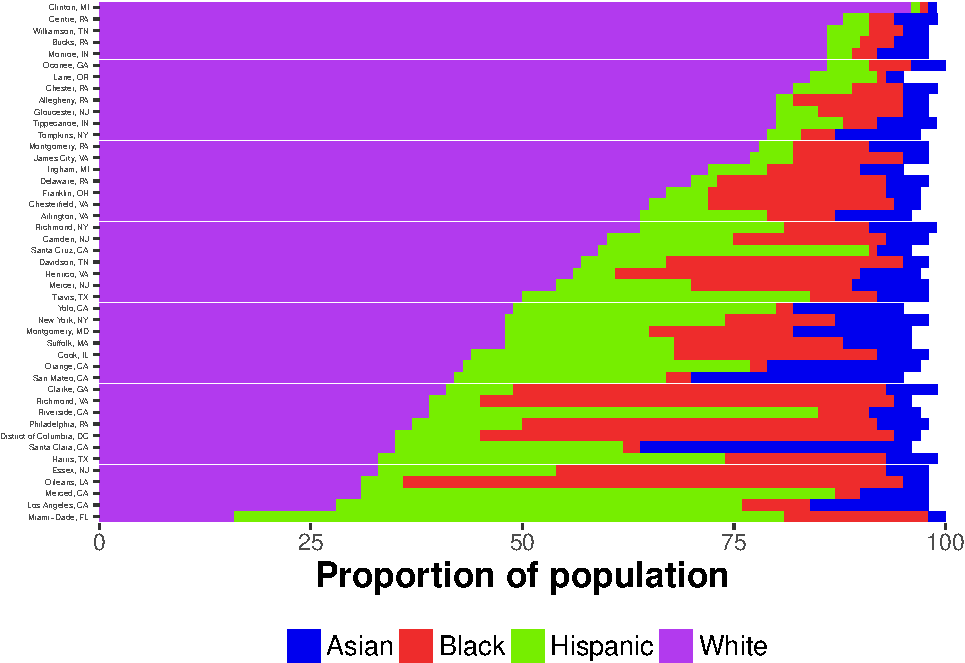
\includegraphics{figs/race-by-county-all-regions-plot-1} 

}

\caption{Racial composition of counties targeted for PLAY project recruitment.}\label{fig:race-by-county}
\end{figure}

\begin{figure}

{\centering 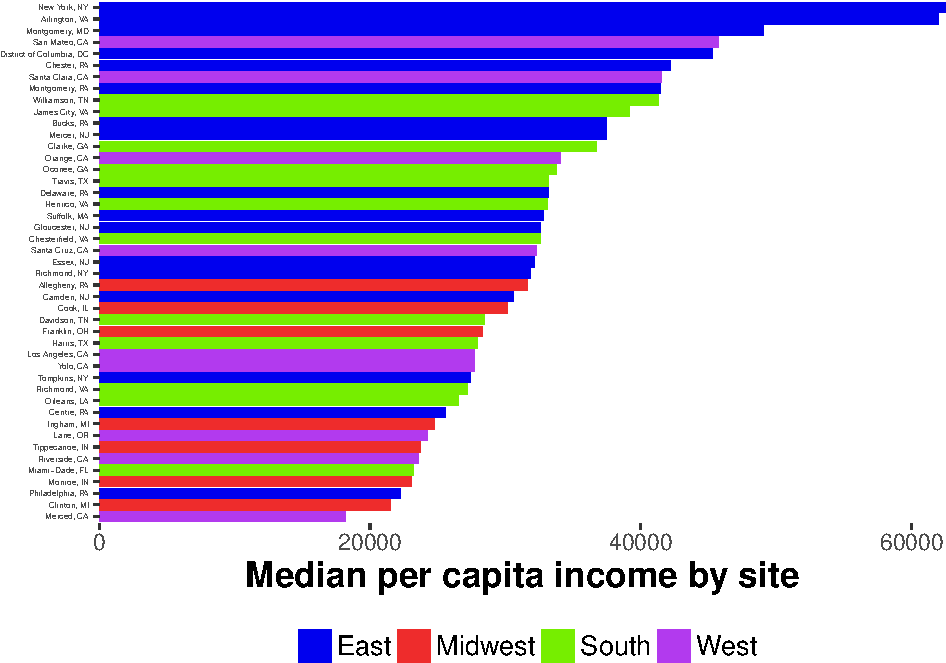
\includegraphics{figs/per-capita-income-plot-1} 

}

\caption{Median per capita income per year in counties targeted for PLAY project recruitment.}\label{fig:PLAY-econ-plot}
\end{figure}

\begin{figure}

{\centering 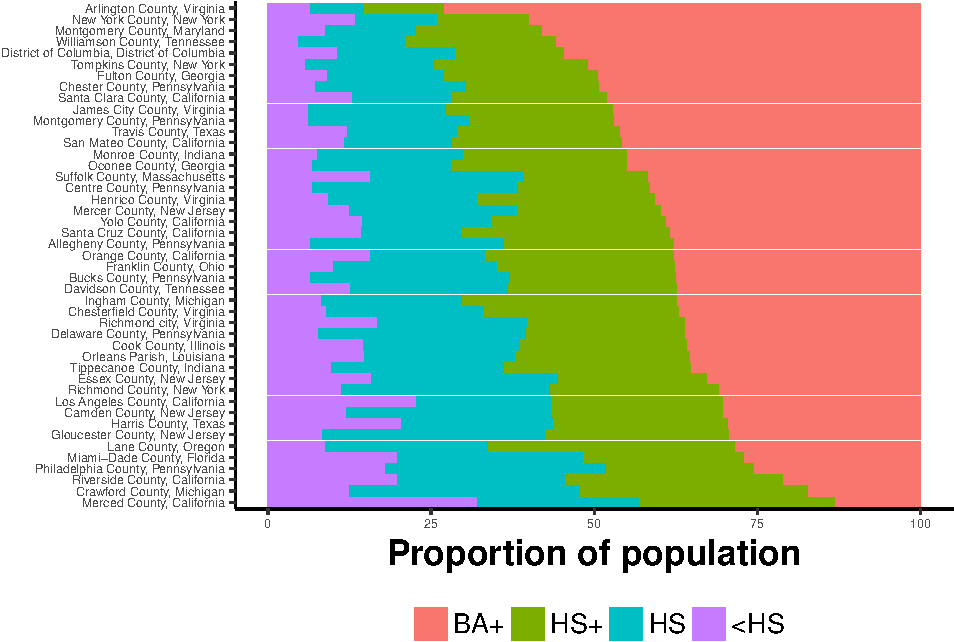
\includegraphics{figs/ed-attain-bars-plot-1} 

}

\caption{Educational attainment in counties targeted for PLAY project recruitment.}\label{fig:PLAY-ed-plot}
\end{figure}

\begin{figure}

{\centering 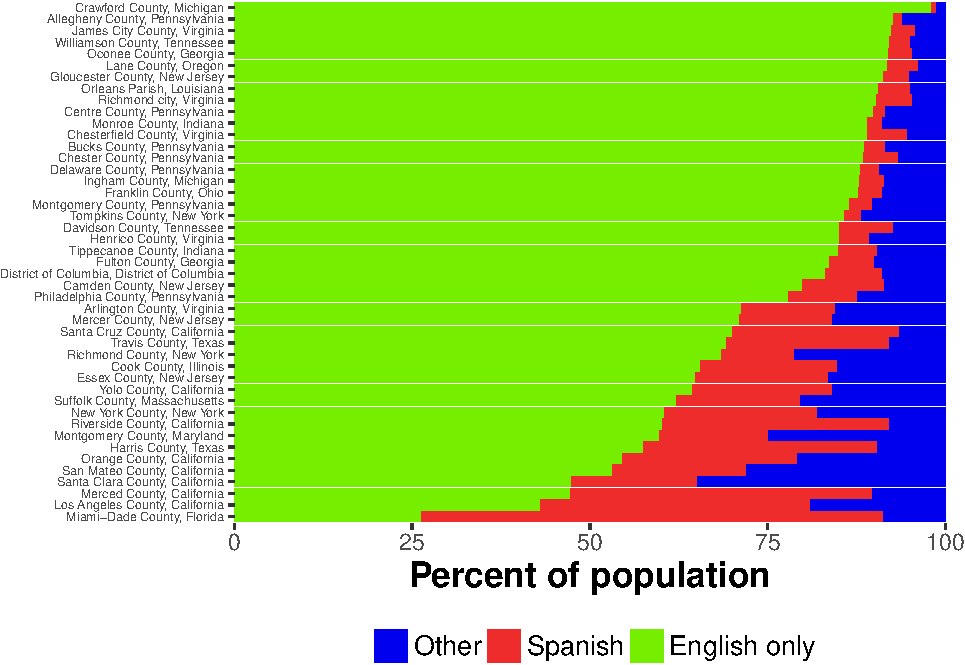
\includegraphics{figs/spanish-speaking-plot-1} 

}

\caption{Proportion of English-only, Spanish, and Other language speakers in counties targeted for PLAY project recruitment.}\label{fig:PLAY-spanish}
\end{figure}

Figure \ref{fig:race-by-county} shows the proportion of African
American, Hispanic/Latino, and Asian residents in the counties
surrounding the collection sites from which participating researchers
will recruit. Figures \ref{fig:PLAY-econ-plot} and
\ref{fig:PLAY-ed-plot} show economic and educational attainment
indicators, respectively. Figure \ref{fig:PLAY-spanish} shows the
proportion of households speaking English-only versus those where
Spanish or other languages are spoken, exclusively or in addition to
English. Data collection sites will have soft, advisory recruiting
targets based on these sorts of measures for their individual
communities.

Families will be two-parent, English and/or Spanish speaking households
with resident fathers, with both parents greater than 18 years of age.
Infants will be term firstborns, without birth complications or
disabilities, and 12, 18, or 24 months of age (±1 week); half of infants
at each age and site will be boys.

The launch group deliberated over several sampling strategies (J. and P.
Bornstein Marc H and Jager, 2013; Davis‐Kean \& Jager, 2017; J. Jager,
Putnick, \& Bornstein, 2017). Ultimately, we decided on homogeneous
sampling to contain costs and understand behavioral variation.
Homogenous sampling maintains some control over sample characteristics
through a set of inclusionary criteria (here, firstborn status,
English/Spanish home language, term pregnancy, etc.), while maximizing
select aspects of diversity (e.g., geography, SES) and retaining
sufficient power for group comparisons. We ruled against conventional
convenience sampling, which leaves sampling decisions entirely to
researchers' discretion. Although convenience sampling is easy and cost
efficient, it risks yielding a sample that varies on too many
demographic dimensions to control. At the other extreme,
population-based (probability) sampling is cost-prohibitive due to the
required sample size. The sheer volume of data would prohibit
transcription and video coding, and would require hiring and training
special researchers for data collection, rather than relying on the
existing expertise of the launch group.

\subsubsection{Procedure}\label{procedure-1}

A publicly-accessible wiki similar to the one used in the pilot (Soska
et al., 2016) will be used to document all procedures and code
definitions.

Based on our experiences with the pilot, we will take several
precautions to minimize effects of experimenter and camera presence on
dyads (McCune-Nicolich, Fenson, \& Others, 1984; Stevenson, Leavitt,
Roach, Chapman, \& Miller, 1986). We will train researchers to remain
unobtrusive. They will stay at a distance, resist talking to mother or
infant, and watch the infant through the viewfinder to avoid eye
contact. Recording will begin after several minutes of infant-mother
acclimation to the camera and researcher.

We plan to collect parent-report measures across multiple domains. For
the \emph{Language} domain, we will use the 12-month (words and
gestures) and 18- to 24-month (words and sentences) versions of the
MacArthur-Bates Communicative Development Inventory (MCDI). The MCDI is
the most widely used instrument of infant language development,
administered to over 60,000 children in 23 languages (Frank, Braginsky,
Yurovsky, \& Marchman, 2017). The 12-month MCDI measures receptive and
expressive vocabulary size and communicative gestures; the 18- to
24-month version contains a larger set of vocabulary items and simple
sentence constructions.

\emph{Locomotion}: Mothers will report the onset ages of hands-knees
crawling and walking, using cell phone videos, photos, and diaries to
jog their memories (Adolph et al., 2012, 2003). QM2: Mothers will report
on infants' fall-related injuries. Infant temperament (QE1) will be
indexed with the Rothbart Early Childhood Behavior Questionnaire (ECBQ),
very short form78,79, which measures dimensions of surgency, negative
affect, and effortful control. Gender (QG1): Mothers will report
infants' use of gender labels (e.g., boy, girl) to refer to themselves
or other people. QG2: Mothers will report their own and the father's
attitudes to gender normative behavior (e.g., \enquote{I would be upset
if my son wanted to dress like a girl}); and household division of labor
(e.g., who does cooking). Environment (NH1): Ambient noise will be
measured during natural play with a decibel meter, placed in the main
room, to record peak and average dB every 100 ms. NH2: In the home video
tour, the researcher will measure room dimensions with a laser distance
measurer. QH3: At the end of the visit, the researcher will fill out a
survey on the home environment (from launch group member Evans). QH4:
Mothers will report use of electronic media (TV, computers, apps, etc.)
by infant and family members (from launch group member Barr). Health
(QF1-4): Mothers will report infant, parent, and family demographics,
infants' health history (based on a subset of questions from the ECLS-B
9-month and 2-year interviews), childcare experience, and parents' and
family health history including SLI, ASD, and mental illnesses.

\subsubsection{Video coding}\label{video-coding-1}

Transcriptions and four core coding passes will be scored for both
infant and mother. PLAY staff will transcribe speech at the utterance
level, using standard criteria for segmenting speech (MacWhinney,
2000b). Utterances will be defined by independent clauses (statements
with subject and predicate) with modifiers. Intonation and pauses can
also define breaks (e.g., \enquote{You like that . Right?} is two
utterances). Mothers' language-like sounds are typed out phonetically.
Infant babbles are marked with \enquote{b} and non-linguistic
vocalizations (cry, laugh, grunt) with \enquote{c.} Unintelligible
utterances are marked \enquote{xxx.} Utterances will be time-locked to
video, revealing overlaps in infant-mother speech, and co-occurrence and
sequencing of speech with object interactions, emotions, and locomotion.
Spanish transcriptions will follow the same rules.

Based on transcripts, mothers' utterances will be coded as declaratives
(labels and descriptions of objects and events \enquote{Red};
\enquote{Puppy}), attention-imperatives that solicit infant attention
(\enquote{Look at that}), action-imperatives that solicit infant action
(\enquote{Put it there}), or prohibition-imperatives (\enquote{Stop
it!}); interrogatives (open- and close-ended questions, \enquote{Is it
hot?} with the exception of \enquote{tag} questions, which will be coded
as declaratives, \enquote{That's a ball, right?});
affirmation/conversational fillers (\enquote{Yes!}; \enquote{What's
next?}), and unintelligible. Infants' vocalizations will be categorized
as language (sentences or words), prelinguistic vocalizations (babbling
or vowels), non-linguistic vocalizations (e.g., cry, laugh, scream,
grunt), or unintelligible.

Gestures will be categorized as points, show/hold up (deictic),
conventional (wave bye-bye, thumbs-up), and representational (flapping
arms to represent a bird).

Object interactions will be coded for onset and offset of manual
engagement (touching, manipulating, carrying) with any manipulable,
moveable object or part of an object that moves through space.
Locomotion will be coded for onset and offset of self-generated
locomotion of any form (e.g., crawling, walking, climbing, stepping in
place). Coders also score falls, and periods when the infant is held or
constrained by furniture (e.g., highchair). Emotion will be coded for
onset and offset of positive (smiling, laughing) and negative (crying,
frowning, fussing) facial expressions. Inter-observer reliability:

To verify inter-observer reliability, PLAY staff will rescore 25\% of
each infant's natural play video (5 minutes randomly drawn from each
20-minute segment), blind to the original coders' output (categorical
measures: kappas \textgreater{}.85; duration measures: \% exact frame
agreement \textgreater{} 90\%). If codes are not reliable, PLAY staff
will reassign the videos to a new lab.

\subsubsection{Data analysis}\label{data-analysis-1}

The launch group will jointly establish best practices for PLAY
analyses. Our guidelines will include: recommendations to pre-register
predictions and analyses; the use of procedures that use one portion of
the data set to explore correlations among variables and a separate
subsample to confirm it; the use of reproducible and transparent
workflows for data processing and analyses (e.g., Ruby scripts in
Datavyu; syntax instead of menu-driven commands for SPSS users; scripts
and functions for R users); a commitment to openly sharing supplementary
video codes and operational definitions to avoid unnecessary duplication
of coding efforts; and open sharing of null results as well as positive
findings. We will create means for communication (e.g., a Google group)
among launch group members who wish to discuss, propose, and organize
team efforts focused on answering specific video-based research
questions. In addition, in keeping with emerging standards in research
transparency (Simmons, Nelson, \& Simonsohn, 2012), we will report how
we determined our sample size, all data exclusions (if any), all
manipulations, and all measures in the study.

\section{General Discussion}\label{general-discussion}

The PLAY corpus will be a treasure trove of data, and it will all be
made available openly to the research community at the end of the study.
Our hope is that it will seed substantial new scholarship.

Researchers can examine real-time behavioral cascades among infant
behaviors, among mother behaviors, and between infants and mothers. They
can test whether particular infant behaviors are temporally connected
(e.g., vocalizations and gestures) or independent (vocalizations and
locomotion). They can test infant-to-mother cascades and vice versa,
such as whether infant emotional expressions affect real-time language
input from mother. Prior correlational work, for example, shows that
infants who express higher quantities of negative emotions display lower
levels of language development on the MCDI and later language milestones
(Bloom \& Capatides, 1987; Salley \& Dixon, 2007). But the evidence for
these findings offers limited insight into the real-time behaviors that
underlie the correlations81 (Bloom \& Beckwith, 1989). With PLAY,
researchers can examine real-time behavioral cascades by testing whether
infants' negative emotions (Table 1 VE1) hinder interactions with
objects (Table 1 VO1) and/or vocal and gestural communications (Table 1
VL2-3), and consequently, lead to low quantity and diversity of mother
speech (Table 1 VL1-2). Infant emotions could also facilitate language
learning: Emotional expressions might elicit mental state terms and
emotion words from mothers (e.g., \enquote{You think mommy's leaving?},
\enquote{Why are you sad?}). Regardless, whether and how infant emotions
affect their language development requires data on the words mothers use
preceding, during, and following infant emotional behaviors in real
time.

PLAY's three age groups and measures of skill and experience (e.g.,
MCDI, walking experience) allow researchers to investigate developmental
cascades in new ways. We can examine age-related changes in temporal
coordination among infant, mother, and infant-mother behaviors---such as
whether infants of different ages with different skills elicit different
behaviors in mothers. For example, object interactions in 12-month-olds,
who are typically at the cusp of conventional word use, might elicit
declaratives from mothers (\enquote{That's a truck!}), whereas object
interactions in 24-month-olds, who typically have substantial expressive
vocabularies, might elicit interrogatives (\enquote{What's that?}).
Alternatively, researchers might compare language cascades in infants of
different ages but with similar skills---whether the vocalizations of
18- versus 24-month-olds matched on MCDI vocabulary size elicit similar
or different language input from mothers. Finally, we might compare
real-time cascades in infants of the same age but with different
skills---such as whether 18-month-olds who use isolated words versus
those who combine words into simple sentences, elicit different language
input from mothers. Comparisons of real-time contingencies by infant age
and skill level provide a unique window into understanding developmental
mechanisms that underpin behavioral change.

Environmental cascades. PLAY's rich array of environmental measures,
ranging from distal macro environmental characteristics (e.g., SES,
geographic region) to proximal environmental features (e.g., clutter and
chaos), will advance understanding of how environmental risks affect
everyday opportunities for learning. Researchers might test proximal
environmental cascades on the quantity and quality of infants' object
interactions and locomotion, for example by coding video home tours
(Table 1 VH1) for object availability and using laser measurements of
room dimensions (Table 2 NH2). We can relate environmental features of
clutter, ambient noise, and so on, to mothers' speech and infants'
language development. Researchers can expand the lens of environmental
influences to consider how distal macro factors, such as family SES and
geo-coded data on neighborhood poverty (Table 2 NH5) relate to proximal
environmental measures---objects and space in the home---and in turn
infant behaviors, mother behaviors, and infant language and skill.

\subsection{Transparency and
reproducibility}\label{transparency-and-reproducibility}

In addition to its scientific innovations, PLAY aims to serve as a model
of how big data science can proceed in a maximally transparent and
reproducible way.

\subsubsection{Data sharing}\label{data-sharing}

All video and self-report data will be openly shared with the research
community on Databrary (``Databrary,'' n.d.), a digital web-based
library for sharing and reusing research videos, clips, and displays
that has received support from NSF, NICHD, SRCD, The Sloan Foundation,
and the LEGO Foundation. Videos associated with all procedures and code
definitions will also be hosted and shared on Databrary and linked to
the wiki. The PLAY launch group will have a short period of exclusive
access to the data before the full dataset is shared in the summer of
2023, at the end of the projected NICHD grant period. By sharing all
data, procedures, and coding information openly, other researchers can
reuse shared videos to ask questions beyond the scope of the original
study (K. E. Adolph, n.d.). They can use shared video clips to learn
about procedures and to illustrate findings and displays for teaching
(Rick O Gilmore \& Adolph, 2017).

Of course, video contains personally identifiable information, so
sharing poses special ethical issues that Databrary's policy framework
solves developed a policy framework53,54 for sharing identifiable data
based on obtaining participants' permission to share and restricting
access to authorized researchers under the oversight of their
institutions.

\subsubsection{Free, open-source tools}\label{free-open-source-tools}

PLAY is committed to using and deploying free and open source tools
wherever possible. Databrary itself is a free and open-source
application (Gilmore \& Simon, n.d.). Datavyu (K. E. Adolph, 2015;
``Welcome!~\textbar{}\textbar{}~datavyu,'' n.d.) is a powerful,
flexible, coding tool that allows researchers to manipulate the
temporal-spatial properties of behavior and to tag portions of the video
for events and behaviors of interest. With fingertip control over video
playback, they can run the video forward and backward at varying speeds
(±1/32- 32x normal speed) or jog frame by frame to determine when
behaviors began and ended, freeze frames to dissect behavior into its
component parts, zoom in/out to focus on details or the larger context,
and label behavioral events with categorical and qualitative codes. Each
code is time-locked to the video to facilitate tests of behavioral
cascades and real-time contingencies based on sequential order,
duration, and begin/end times of events. A full scripting language
allows researchers to manipulate the spreadsheet, error-check entries,
import other data streams, and export data to their specifications for
analyses. The latest Datavyu release has new features to reduce the
notoriously high cost of transcribing infant and mother speech in noisy
contexts, time locked to video, at the utterance level (from the typical
10-12 hours per hour of video to 7-9 hours).

\subsubsection{Open, transparent, and reproducible
workflows}\label{open-transparent-and-reproducible-workflows}

We have already begun to develop and deploy reproducible workflows using
R. A repository on Github (PLAY-behaviorome) has been created to house
processing scripts for the PLAY data (Gilmore, n.d.) including analyses
of the PLAY launch group members characteristics, characteristics of the
data collection sites, and so on. Indeed, the summary statistics about
the PLAY Launch Group and the pilot study participants were derived
directly from raw data files and incorporated into this manuscript using
the \texttt{papaja} package (Aust \& Barth, 2017) we used to create the
paper. The PLAY-behaviorome repository includes the newly released alpha
version of the \texttt{databraryapi} R package (Gilmore, 21AD) for
interacting with Databrary from within R. We welcome community input on
the package, and we plan to improve the package over time. We will
eventually release a Python version, as well. In addition, this paper's
analyses and plots can be re-generated from the repository associated
with the working manuscript (``PLAY project protocol manuscript,''
n.d.).

\subsubsection{Reducing false-positives and
pre-registration}\label{reducing-false-positives-and-pre-registration}

Naturally, The creation of a large dataset with many variables raises
the possibility that a particular statistically significant finding may
be spurious. In particular, correlational analyses among non-video
questionnaire data require special protection against spurious findings
because of the large number of easily available measures (Table 2). The
corpus includes a summary score for each infant on each instrument,
subscores for standard scales, and raw data for each item. For example,
researchers will have access to infants' total productive vocabulary on
the MCDI, the number of words produced within specific categories (e.g.,
animal words; action words), and production of each word. Similarly,
researchers will have access to fully processed, ready-to-analyze data
on infant temperament, locomotor experience, infant health,
environmental chaos, media use, family demographics, and so on. Spurious
results and duplication of analyses are especially likely from these
\enquote{low-hanging fruit.}

In contrast to the ready-to-use questionnaire data, analyses of
time-locked video codes raise other analytic issues. Data from the
foundational coding passes will not be \enquote{ready to go.}
Researchers will need to make decisions about how to process the
data---whether to turn categorical codes into frequencies or rates;
whether to convert onset/offset times into average durations, latencies
from one behavior to another, sequences of behavior, or other analytic
constructs. We will encourage individual launch group members to use
their expertise and Datavyu training to mine the video corpus (by
further coding of natural play and coding of structured play sessions
and the home tour). Additional coding passes will be labor intensive,
and duplication of coding effort would waste researchers' time.

Of course, PLAY's homogenous sampling strategy and cross-sectional
design have limitations. Although the sample will not be nationally
representative, it will capture important demographic variations and can
easily grow. With only one session per dyad, we cannot test stability or
predictive validity of behaviors. However, the protocol and codes can be
easily extended to other populations and to longitudinal designs
(several launch group members plan to do this). If labs assigned to data
collection or coding cannot fulfill their tasks, we will replace them.\\
We will monitor ongoing data collections. If the data are too
homogeneous, we will ask some sites to recruit more than their
allotment. If a lab's codes are not reliable, we will reassign the
videos and retrain the coder.

\subsection{Conclusion}\label{conclusion}

In conclusion, the PLAY project represents an innovative, synergistic,
cross-domain approach to developmental science that will facilitate
scientific discovery, transparency, and reproducibility we hope for
years to come. In creating the first, large-scale, sharable, reusable,
fully transcribed, coded, and curated video corpus of human behavior, we
hope to establish video sharing of procedures, codes, and findings as a
new standard in developmental and behavioral science. In so doing, we
hope to help answer fundamental cross-domain questions about behavioral,
environmental, and developmental cascades as they shape the playful work
of infants.

\newpage

\section{References}\label{references}

\setlength{\parindent}{-0.5in} \setlength{\leftskip}{0.5in}

\hypertarget{refs}{}
\hypertarget{ref-Adolph2015-oy}{}
Adolph, K. E. (2015). Best practices for coding behavioral data from
video. \url{http://datavyu.org/user-guide/best-practices.html}.
Retrieved from \url{http://datavyu.org/user-guide/best-practices.html}

\hypertarget{ref-Adolph_undated-od}{}
Adolph, K. E. (n.d.).
Video~as~data:~from~transient~behavior~to~tangible~recording.
\emph{APS~Observer}, in press.

\hypertarget{ref-Adolph2012-ab}{}
Adolph, K. E., Cole, W. G., Komati, M., Garciaguirre, J. S., Badaly, D.,
Lingeman, J. M., \ldots{} Sotsky, R. B. (2012). How do you learn to
walk? Thousands of steps and dozens of falls per day.
\emph{Psychological Science}, \emph{23}(11), 1387--1394.
doi:\href{https://doi.org/10.1177/0956797612446346}{10.1177/0956797612446346}

\hypertarget{ref-Adolph2017-ac}{}
Adolph, K. E., Gilmore, R. O., \& Kennedy, J. L. (2017, October). Video
data and documentation will improve psychological science.
\url{http://www.apa.org/science/about/psa/2017/10/video-data.aspx}.
Retrieved from
\url{http://www.apa.org/science/about/psa/2017/10/video-data.aspx}

\hypertarget{ref-PLAY-workshop-Databrary}{}
Adolph, K. E., Gilmore, R. O., \& Tamis-LeMonda, C. (2016). Play \&
learning across a year (PLAY) workshop at NICHD.
\url{https://nyu.databrary.org/volume/254}.
doi:\href{https://doi.org/10.17910/B7.254}{10.17910/B7.254}

\hypertarget{ref-PLAY-pilot-volume}{}
Adolph, K. E., Gilmore, R. O., \& Tamis-LeMonda, C. (2018, March). PLAY
pilot data collections. \url{https://nyu.databrary.org/volume/444}.
Retrieved from \url{https://nyu.databrary.org/volume/444}

\hypertarget{ref-PLAY-webinar-Databrary}{}
Adolph, K. E., Tamis-LeMonda, C. L., \& Gilmore, R. O. (n.d.). PLAY
project: Webinar discussions on protocol and coding.
\url{https://nyu.databrary.org/volume/232}. Retrieved from
\url{https://nyu.databrary.org/volume/232}

\hypertarget{ref-play-pilot-volume}{}
Adolph, K. E., Tamis-LeMonda, Catherine, \& Gilmore, R. O. (n.d.). PLAY
pilot data collections. Retrieved from
\url{https://nyu.databrary.org/volume/444.}

\hypertarget{ref-Adolph2003-rw}{}
Adolph, K. E., Vereijken, B., \& Shrout, P. E. (2003). What changes in
infant walking and why. \emph{Child Development}, \emph{74}(2),
475--497. Retrieved from
\url{https://www.ncbi.nlm.nih.gov/pubmed/12705568}

\hypertarget{ref-R-papaja}{}
Aust, F., \& Barth, M. (2017). \emph{papaja: Create APA manuscripts with
R Markdown}. Retrieved from \url{https://github.com/crsh/papaja}

\hypertarget{ref-De_Barbaro2015-bp}{}
Barbaro, K. de, Johnson, C. M., Forster, D., \& Deák, G. O. (2015).
Sensorimotor decoupling contributes to triadic attention: A longitudinal
investigation of Mother-Infant-Object interactions. \emph{Child
Development}, \emph{87}(2), 494--512.
doi:\href{https://doi.org/10.1111/cdev.12464}{10.1111/cdev.12464}

\hypertarget{ref-Bloom1995-xb}{}
Bloom, L. (1995).
\emph{The~transition~from~infancy~to~language:~acquiring~the~power~of
expression}. Cambridge~University~Press. Retrieved from
\url{https://market.android.com/details?id=book-ntvdZv1wttQC}

\hypertarget{ref-Bloom1989-mw}{}
Bloom, L., \& Beckwith, R. (1989). Talking with feeling: Integrating
affective and linguistic expression in early language development.
\emph{Cognition and Emotion}, \emph{3}(4), 313--342.
doi:\href{https://doi.org/10.1080/02699938908412711}{10.1080/02699938908412711}

\hypertarget{ref-Bloom1987-md}{}
Bloom, L., \& Capatides, J. B. (1987). Expression of affect and the
emergence of language. \emph{Child Development}, \emph{58}(6),
1513--1522. doi:\href{https://doi.org/10.2307/1130691}{10.2307/1130691}

\hypertarget{ref-Bornstein2013-mr}{}
Bornstein, J. and P., Marc H and Jager. (2013).
Sampling~in~developmental~science:~situations,~shortcomings,
~~~solutions,~and~standards. \emph{Developmental~Review:~DR},
\emph{33}(4), 357--370.
doi:\href{https://doi.org/10.1016/j.dr.2013.08.003}{10.1016/j.dr.2013.08.003}

\hypertarget{ref-Bruner1975-sp}{}
Bruner, J. S. (1975). Play~is~serious~business. \emph{Psychology~Today},
\emph{8}(8), 80--83.

\hypertarget{ref-Bruner1976-ab}{}
Bruner, J. S. (1976).
\emph{Play,~its~role~in~development~and~evolution}. Basic~Books.
Retrieved from
\url{https://market.android.com/details?id=book-Zq8oAAAAYAAJ}

\hypertarget{ref-Cole2012-vr}{}
Cole, W. G., Lingeman, J. M., \& Adolph, K. E. (2012). Go naked: Diapers
affect infant walking. \emph{Developmental Science}, \emph{15}(6),
783--790.
doi:\href{https://doi.org/10.1111/j.1467-7687.2012.01169.x}{10.1111/j.1467-7687.2012.01169.x}

\hypertarget{ref-databrary-site}{}
Databrary. (n.d.). \url{https://nyu.databrary.org/}. Retrieved from
\url{https://nyu.databrary.org/}

\hypertarget{ref-DavisKean2017-sr}{}
Davis‐Kean, P. E., \& Jager, J. (2017). From small to big: Methods for
incorporating large scale data into developmental science.
\emph{Monographs of the Society for Research in Child Development}.
Retrieved from
\url{http://onlinelibrary.wiley.com/doi/10.1111/mono.12297/full}

\hypertarget{ref-Fausey2016-kx}{}
Fausey, C. M., Jayaraman, S., \& Smith, L. B. (2016). From faces to
hands: Changing visual input in the first two years. \emph{Cognition},
\emph{152}, 101--107.
doi:\href{https://doi.org/10.1016/j.cognition.2016.03.005}{10.1016/j.cognition.2016.03.005}

\hypertarget{ref-Frank2017-tb}{}
Frank, M. C., Bergelson, E., Bergmann, C., Cristia, A., Floccia, C.,
Gervain, J., \ldots{} Others. (2017). A collaborative approach to infant
research: Promoting reproducibility, best practices, and
Theory-Building. \emph{Infancy: The Official Journal of the
International Society on Infant Studies}. Retrieved from
\url{http://onlinelibrary.wiley.com/doi/10.1111/infa.12182/full}

\hypertarget{ref-Frank2017-bt}{}
Frank, M. C., Braginsky, M., Yurovsky, D., \& Marchman, V. A. (2017).
Wordbank: An open repository for developmental vocabulary data.
\emph{Journal of Child Language}, \emph{44}(3), 677--694.
doi:\href{https://doi.org/10.1017/S0305000916000209}{10.1017/S0305000916000209}

\hypertarget{ref-Gesell1946-qr}{}
Gesell, A. (1946). Cinematography~and~the~study~of~child~development.
\emph{The~American~Naturalist}, \emph{80}(793), 470--475. Retrieved from
\url{http://www.jstor.org/stable/2458189}

\hypertarget{ref-Gesell1991-sx}{}
Gesell, A. (1991). Cinemanalysis:~a~method~of~behavior~study.
\emph{The~Journal~of~Genetic~Psychology}, \emph{152}(4), 549--562.
doi:\href{https://doi.org/10.1080/00221325.1991.9914712}{10.1080/00221325.1991.9914712}

\hypertarget{ref-Gibson1994-kb}{}
Gibson, E. J. (1994). Has psychology a future? \emph{Psychological
Science}, \emph{5}(2), 69--76.
doi:\href{https://doi.org/10.1111/j.1467-9280.1994.tb00633.x}{10.1111/j.1467-9280.1994.tb00633.x}

\hypertarget{ref-databraryapi}{}
Gilmore, R. O. (21AD). databraryapi: An r package for databrary.
Retrieved from \url{https://github.com/PLAY-behaviorome/databraryapi}

\hypertarget{ref-R-databraryapi}{}
Gilmore, R. O. (21AD). \emph{databraryapi: An r package for databrary}.
Retrieved from \url{https://github.com/PLAY-behaviorome/databraryapi}

\hypertarget{ref-cite-PLAY-behaviorome}{}
Gilmore, R. O. (n.d.). PLAY project protocol manuscript. Retrieved from
\url{https://github.com/PLAY-behaviorome/}

\hypertarget{ref-Gilmore2017-eh}{}
Gilmore, R. O., \& Adolph, K. E. (2017). Video can make behavioural
science more reproducible. \emph{Nature Human Behavior}, \emph{1}.
doi:\href{https://doi.org/10.1038/s41562-017-0128}{10.1038/s41562-017-0128}

\hypertarget{ref-Gilmore_undated-tp}{}
Gilmore, R. O., \& Adolph, K. E. (n.d.). \emph{Open sharing of research
video: Breaking the boundaries of the research team, in advancing social
and behavioral health research through cross-disciplinary team science:
Principles for success}. (Hall, Kara, Croyle, R., \& Vogel, A., Ed.).
Springer.

\hypertarget{ref-databrary-release}{}
Gilmore, R. O., \& Adolph, K. E. (n.d.). Video data release template,
participants \textbar{}\textbar{} databrary: An open data library for
developmental science.
\url{https://www.databrary.org/resources/templates/release-template.html}.
Retrieved from
\url{https://www.databrary.org/resources/templates/release-template.html}

\hypertarget{ref-databrary-on-github}{}
Gilmore, R. O., \& Simon, D. (n.d.). \emph{Databrary repository on
GitHub}. Retrieved from \url{https://github.com/databrary}

\hypertarget{ref-Gilmore2016-ev}{}
Gilmore, R. O., Adolph, K. E., \& Millman, D. S. (2016). Curating
identifiable data for sharing: The databrary project. In \emph{2016 new
york scientific data summit (NYSDS)} (pp. 1--6). ieeexplore.ieee.org.
doi:\href{https://doi.org/10.1109/NYSDS.2016.7747817}{10.1109/NYSDS.2016.7747817}

\hypertarget{ref-Gilmore2016-wl}{}
Gilmore, R. O., Adolph, K. E., Millman, D. S., \& Gordon, A. (2016).
Transforming education research through open video data sharing.
\emph{Advances in Engineering Education}, \emph{5}(2). Retrieved from
\url{https://www.ncbi.nlm.nih.gov/pubmed/28042361}

\hypertarget{ref-R-acs}{}
Glenn, E. H. (2018). \emph{Acs: Download, manipulate, and present
american community survey and decennial data from the us census}.
Retrieved from \url{https://CRAN.R-project.org/package=acs}

\hypertarget{ref-Halim2013-ez}{}
Halim, M. L., Ruble, D., Tamis-LeMonda, C., \& Shrout, P. E. (2013).
Rigidity in gender-typed behaviors in early childhood: A longitudinal
study of ethnic minority children. \emph{Child Development},
\emph{84}(4), 1269--1284.
doi:\href{https://doi.org/10.1111/cdev.12057}{10.1111/cdev.12057}

\hypertarget{ref-R-purrr}{}
Henry, L., \& Wickham, H. (2017). \emph{Purrr: Functional programming
tools}. Retrieved from \url{https://CRAN.R-project.org/package=purrr}

\hypertarget{ref-Hoff2013-er}{}
Hoff, E. (2013). \emph{Language~development}. Cengage~Learning.
Retrieved from
\url{https://market.android.com/details?id=book-7MxTSQlfUVUC}

\hypertarget{ref-Iverson2007-yr}{}
Iverson, J. M., \& Wozniak, R. H. (2007). Variation in vocal-motor
development in infant siblings of children with autism. \emph{Journal of
Autism and Developmental Disorders}, \emph{37}(1), 158--170.
doi:\href{https://doi.org/10.1007/s10803-006-0339-z}{10.1007/s10803-006-0339-z}

\hypertarget{ref-Jager2017-wv}{}
Jager, J., Putnick, D. L., \& Bornstein, M. H. (2017). More than just
convenient: The scientific merits of homogeneous convenience samples.
\emph{Monographs of the Society for Research in Child Development},
\emph{82}(2), 13--30.
doi:\href{https://doi.org/10.1111/mono.12296}{10.1111/mono.12296}

\hypertarget{ref-R-chron}{}
James, D., \& Hornik, K. (2018). \emph{Chron: Chronological objects
which can handle dates and times}. Retrieved from
\url{https://CRAN.R-project.org/package=chron}

\hypertarget{ref-R-ggmap}{}
Kahle, D., \& Wickham, H. (2013). Ggmap: Spatial visualization with
ggplot2. \emph{The R Journal}, \emph{5}(1), 144--161. Retrieved from
\url{http://journal.r-project.org/archive/2013-1/kahle-wickham.pdf}

\hypertarget{ref-Karasik2012-jq}{}
Karasik, L. B., Adolph, K. E., Tamis-LeMonda, C. S., \& Zuckerman, A. L.
(2012). Carry on: Spontaneous object carrying in 13-month-old crawling
and walking infants. \emph{Developmental Psychology}, \emph{48}(2),
389--397. doi:\href{https://doi.org/10.1037/a0026040}{10.1037/a0026040}

\hypertarget{ref-Karasik2011-mf}{}
Karasik, L. B., Tamis-LeMonda, C. S., \& Adolph, K. E. (2011).
Transition from crawling to walking and infants' actions with objects
and people. \emph{Child Development}, \emph{82}(4), 1199--1209.
doi:\href{https://doi.org/10.1111/j.1467-8624.2011.01595.x}{10.1111/j.1467-8624.2011.01595.x}

\hypertarget{ref-Karasik2014-cd}{}
Karasik, L. B., Tamis-Lemonda, C. S., \& Adolph, K. E. (2014). Crawling
and walking infants elicit different verbal responses from mothers.
\emph{Developmental Science}, \emph{17}(3), 388--395.
doi:\href{https://doi.org/10.1111/desc.12129}{10.1111/desc.12129}

\hypertarget{ref-Karasik2015-mi}{}
Karasik, L. B., Tamis-LeMonda, C. S., Adolph, K. E., \& Bornstein, M. H.
(2015). Places and postures: A cross-cultural comparison of sitting in
5-month-olds. \emph{Journal of Cross-Cultural Psychology}, \emph{46}(8),
1023--1038.
doi:\href{https://doi.org/10.1177/0022022115593803}{10.1177/0022022115593803}

\hypertarget{ref-R-choroplethrMaps}{}
Lamstein, A. (2017). \emph{ChoroplethrMaps: Contains maps used by the
'choroplethr' package}. Retrieved from
\url{https://CRAN.R-project.org/package=choroplethrMaps}

\hypertarget{ref-R-choroplethr}{}
Lamstein, A., \& Johnson, B. P. (2017). \emph{Choroplethr: Simplify the
creation of choropleth maps in r}. Retrieved from
\url{https://CRAN.R-project.org/package=choroplethr}

\hypertarget{ref-R-XML}{}
Lang, D. T., \& CRAN Team. (2018). \emph{XML: Tools for parsing and
generating xml within r and s-plus}. Retrieved from
\url{https://CRAN.R-project.org/package=XML}

\hypertarget{ref-MacWhinney2000-yn}{}
MacWhinney, B. (2000a). The CHILDES project: Tools for analyzing talk
(third edition): Volume i: Transcription format and programs, volume II:
The database. \emph{Computational Linguistics}, \emph{26}(4), 657--657.
doi:\href{https://doi.org/10.1162/coli.2000.26.4.657}{10.1162/coli.2000.26.4.657}

\hypertarget{ref-MacWhinney2000-fb}{}
MacWhinney, B. (2000b). \emph{The CHILDES project: Tools for analyzing
talk}. Lawrence Erlbaum Associates.
doi:\href{https://doi.org/10.1162/coli.2000.26.4.657}{10.1162/coli.2000.26.4.657}

\hypertarget{ref-McCune-Nicolich1984-tn}{}
McCune-Nicolich, L., Fenson, L., \& Others. (1984). Methodological
issues in studying early pretend play. \emph{Child's Play: Developmental
and Applied}, 81--104.

\hypertarget{ref-Montessori1984-la}{}
Montessori, M. (1984). \emph{The~absorbent~mind}. New~York:
Dell~Publishing~Co.,~Inc. Retrieved from
\url{https://openlibrary.org/books/OL22287831M.opds}

\hypertarget{ref-R-bindrcpp}{}
Müller, K. (2016). \emph{Bindrcpp: An 'rcpp' interface to active
bindings}. Retrieved from
\url{https://CRAN.R-project.org/package=bindrcpp}

\hypertarget{ref-Onis2006-le}{}
Onis, M. (2006).
WHO~motor~development~study:~windows~of~achievement~for~six
gross~motor~development~milestones. \emph{Acta~Paediatrica},
\emph{95}(S450), 86--95. Retrieved from
\url{http://onlinelibrary.wiley.com/doi/10.1111/j.1651-2227.2006.tb02379.x/full}

\hypertarget{ref-R-jsonlite}{}
Ooms, J. (2014). The jsonlite package: A practical and consistent
mapping between json data and r objects. \emph{arXiv:1403.2805
{[}Stat.CO{]}}. Retrieved from \url{https://arxiv.org/abs/1403.2805}

\hypertarget{ref-Piaget1967-nl}{}
Piaget, J. (1967). \emph{Play,~dreams~and~imitation~in~childhood}.
London: Routledge~\&~K.~Paul. Retrieved from
\url{https://openlibrary.org/books/OL22344377M.opds}

\hypertarget{ref-ibad-PLAY-github}{}
PLAY project protocol manuscript. (n.d.). Retrieved from
\url{https://github.com/PLAY-behaviorome/ibad-lets-PLAY}

\hypertarget{ref-R-base}{}
R Core Team. (2017). \emph{R: A language and environment for statistical
computing}. Vienna, Austria: R Foundation for Statistical Computing.
Retrieved from \url{https://www.R-project.org/}

\hypertarget{ref-Robinson2015-qe}{}
Robinson, A. K. \&., SR. (2015). Motor~development. In
\emph{Handbook~of~child~psychology~and~developmental~science} (Vol. 2,
pp. 114--157). Hoboken,~NJ,~USA: John~Wiley~\&~Sons,~Inc.
doi:\href{https://doi.org/10.1002/9781118963418.childpsy204}{10.1002/9781118963418.childpsy204}

\hypertarget{ref-Rowe2012-vy}{}
Rowe, M. L. (2012). A longitudinal investigation of the role of quantity
and quality of child-directed speech in vocabulary development.
\emph{Child Development}, \emph{83}(5), 1762--1774.
doi:\href{https://doi.org/10.1111/j.1467-8624.2012.01805.x}{10.1111/j.1467-8624.2012.01805.x}

\hypertarget{ref-Salley2007-gz}{}
Salley, B. J., \& Dixon, W. E., Jr. (2007). Temperamental and joint
attentional predictors of language development. \emph{Merrill-Palmer
Quarterly}, \emph{53}(1), 131--154. Retrieved from
\url{https://www.ncbi.nlm.nih.gov/pubmed/18080005}

\hypertarget{ref-Simmons2012-ma}{}
Simmons, J. P., Nelson, L. D., \& Simonsohn, U. (2012). A 21 word
solution.
doi:\href{https://doi.org/10.2139/ssrn.2160588}{10.2139/ssrn.2160588}

\hypertarget{ref-Soderstrom2013-xn}{}
Soderstrom, M., \& Wittebolle, K. (2013). When do caregivers talk? The
influences of activity and time of day on caregiver speech and child
vocalizations in two childcare environments. \emph{PloS One},
\emph{8}(11), e80646.
doi:\href{https://doi.org/10.1371/journal.pone.0080646}{10.1371/journal.pone.0080646}

\hypertarget{ref-Soska2016-yo}{}
Soska, K., Adolph, K. E., Tamis-LeMonda, C., \& Gilmore, R. O. (2016,
December). The PLAY project wiki.
\url{https://dev1.ed-projects.nyu.edu/wikis/docuwiki/doku.php}.
Retrieved from
\url{https://dev1.ed-projects.nyu.edu/wikis/docuwiki/doku.php}

\hypertarget{ref-Stevenson1986-zh}{}
Stevenson, M. B., Leavitt, L. A., Roach, M. A., Chapman, R. S., \&
Miller, J. F. (1986). Mothers' speech to their 1-year-old infants in
home and laboratory settings. \emph{Journal of Psycholinguistic
Research}, \emph{15}(5), 451--461.
doi:\href{https://doi.org/10.1007/BF01067725}{10.1007/BF01067725}

\hypertarget{ref-datavyu-site}{}
Welcome!~\textbar{}\textbar{}~datavyu:~video~coding~and~data~visualization~tool.
(n.d.). \url{http://datavyu.org}. Retrieved from
\url{http://datavyu.org}

\hypertarget{ref-R-ggplot2}{}
Wickham, H. (2009). \emph{Ggplot2: Elegant graphics for data analysis}.
Springer-Verlag New York. Retrieved from \url{http://ggplot2.org}

\hypertarget{ref-R-httr}{}
Wickham, H. (2017a). \emph{Httr: Tools for working with urls and http}.
Retrieved from \url{https://CRAN.R-project.org/package=httr}

\hypertarget{ref-R-tidyr}{}
Wickham, H. (2017b). \emph{Tidyr: Easily tidy data with 'spread()' and
'gather()' functions}. Retrieved from
\url{https://CRAN.R-project.org/package=tidyr}

\hypertarget{ref-R-tidyverse}{}
Wickham, H. (2017c). \emph{Tidyverse: Easily install and load
'tidyverse' packages}. Retrieved from
\url{https://CRAN.R-project.org/package=tidyverse}

\hypertarget{ref-R-forcats}{}
Wickham, H. (2018a). \emph{Forcats: Tools for working with categorical
variables (factors)}. Retrieved from
\url{https://CRAN.R-project.org/package=forcats}

\hypertarget{ref-R-stringr}{}
Wickham, H. (2018b). \emph{Stringr: Simple, consistent wrappers for
common string operations}. Retrieved from
\url{https://CRAN.R-project.org/package=stringr}

\hypertarget{ref-R-dplyr}{}
Wickham, H., \& Francois, R. (2016). \emph{Dplyr: A grammar of data
manipulation}. Retrieved from
\url{https://CRAN.R-project.org/package=dplyr}

\hypertarget{ref-R-tibble}{}
Wickham, H., Francois, R., \& Müller, K. (2017). \emph{Tibble: Simple
data frames}. Retrieved from
\url{https://CRAN.R-project.org/package=tibble}

\hypertarget{ref-R-readr}{}
Wickham, H., Hester, J., \& Francois, R. (2017). \emph{Readr: Read
rectangular text data}. Retrieved from
\url{https://CRAN.R-project.org/package=readr}






\end{document}
